\documentclass{article}
\usepackage{tikz}
\usepackage{amssymb}
\pagestyle{empty}
\begin{document}
% GEOMIRA export: TikZ. One unit is 28.571429bp (38.095238 px on screen).
% Needs \usepackage{tikz} and \usepackage{amssymb}.
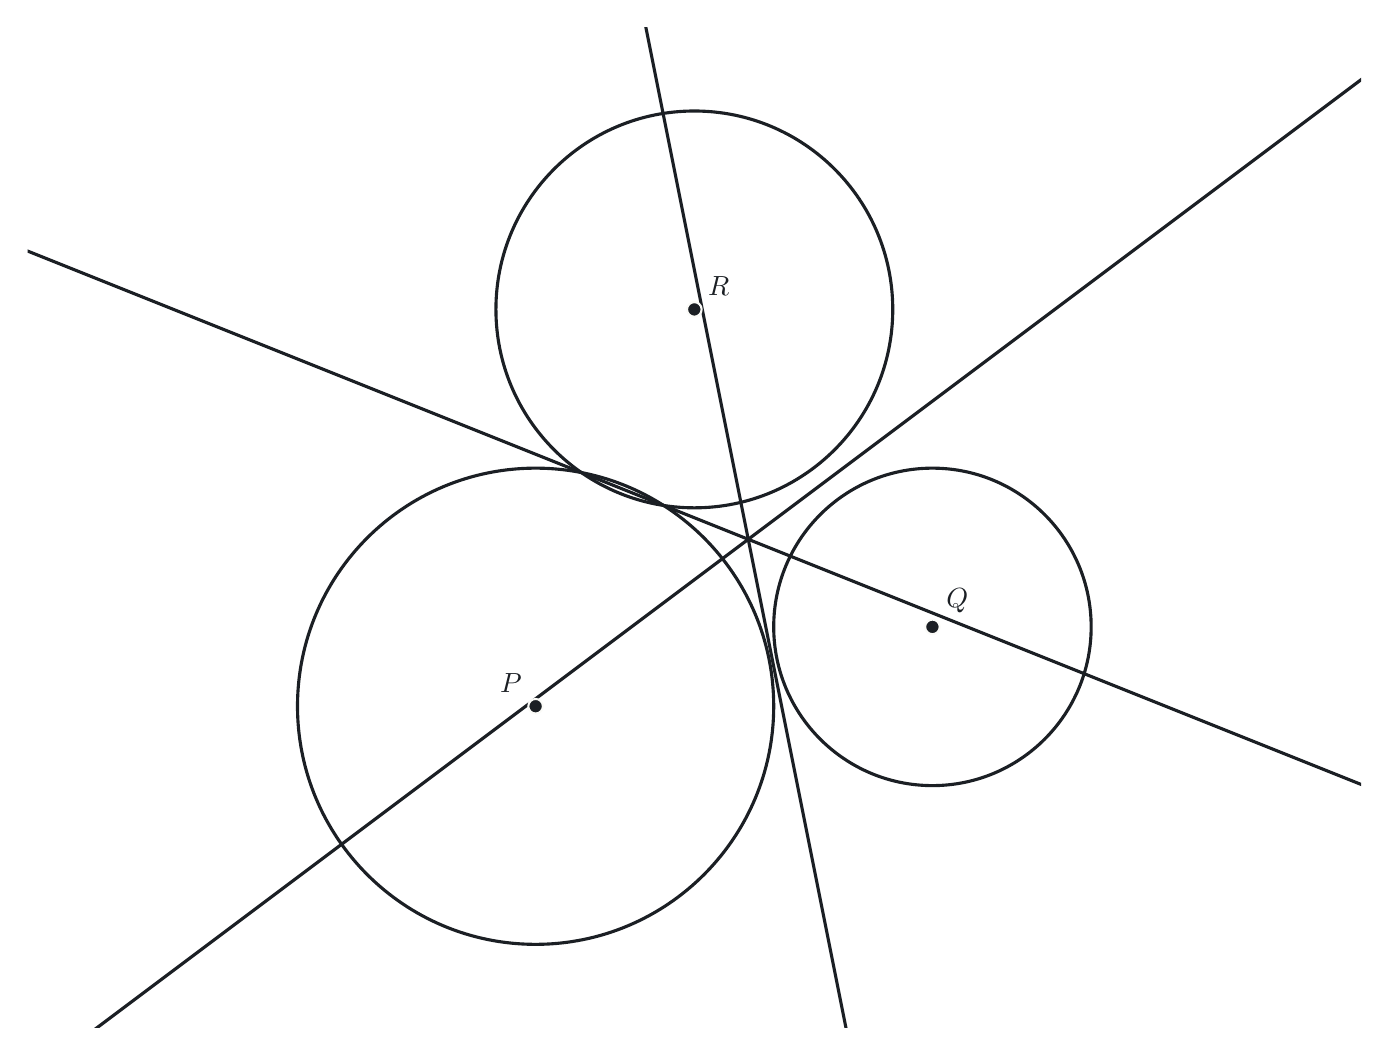
\begin{tikzpicture}[x=28.571429bp, y=28.571429bp, line cap=round, line join=round]
\definecolor{gmc0}{HTML}{1B1F24}
\definecolor{gmc1}{HTML}{FBFBF8}
\clip (-6.4,-4.05) rectangle (10.4,8.55);
% c1
\draw[gmc0, line width=1.125bp] (3,0) arc[start angle=0, end angle=360, radius=3];
% c2
\draw[gmc0, line width=1.125bp] (7,1) arc[start angle=0, end angle=360, radius=2];
% c3
\draw[gmc0, line width=1.125bp] (4.5,5) arc[start angle=0, end angle=360, radius=2.5];
% r12
\draw[gmc0, line width=1.125bp] (4.267,-5.835) -- (1.033,10.335);
% r23
\draw[gmc0, line width=1.125bp] (12.185,9.2325) -- (-7.905,-5.835);
% r13
\draw[gmc0, line width=1.125bp] (12.185,-1.699) -- (-8.185,6.449);
% P
\filldraw[fill=gmc0, draw=gmc1, line width=0.75bp] (0,0) circle[radius=2.625bp];
% Q
\filldraw[fill=gmc0, draw=gmc1, line width=0.75bp] (5,1) circle[radius=2.625bp];
% R
\filldraw[fill=gmc0, draw=gmc1, line width=0.75bp] (2,5) circle[radius=2.625bp];
\node[anchor=south east, inner sep=0pt, text=gmc0] at (-0.1671,0.1671) {$P$}; % label of P
\node[anchor=south west, inner sep=0pt, text=gmc0] at (5.1671,1.1671) {$Q$}; % label of Q
\node[anchor=south west, inner sep=0pt, text=gmc0] at (2.1671,5.1671) {$R$}; % label of R
\end{tikzpicture}

\end{document}
